\chapter{Function verification}
To verify the functionality of the device, a serie of basic measurements was performed. Later on a more complex test - injecting synthetised pulses to the fastic - was performed and the functionality of the whole device was thus verified.
\section{Measurements}
Multiple measurements were done to verify the basic functionality of the device. A \SI{200}{\mega\hertz} DSO-X 2024A oscilloscobe with a \SI{350}{\mega\hertz} probe has been used to carry out the measurements. Measurements on the power supplies were done as close to the supply output as possible. A spring contact was used to contact the ground of the probe to minimize the loop inductance of the probe.
\subsection{Power supplies}
The output ripple of the step down DC/DC converter was measured to be \SI{26}{\milli\volt} peak-to-peak. The frequency of the ripple measured coresponds well to the switching frequency of the converter (\SI{750}{\kilo\hertz}) \cite{diodes_ap62201} which can be seen in Figure \ref{fig:dcdc_ripple}. Note that the cursor frequency is measured over the span of 5 periods to get better accuracy, thus the measured value has to be multiplied by 5. For the LDOs, there was no observable ripple on the output. Both of these confirm that the power network integrity of the device is very good.

\FloatBarrier
\begin{figure}[!htpb]
    \begin{center}
        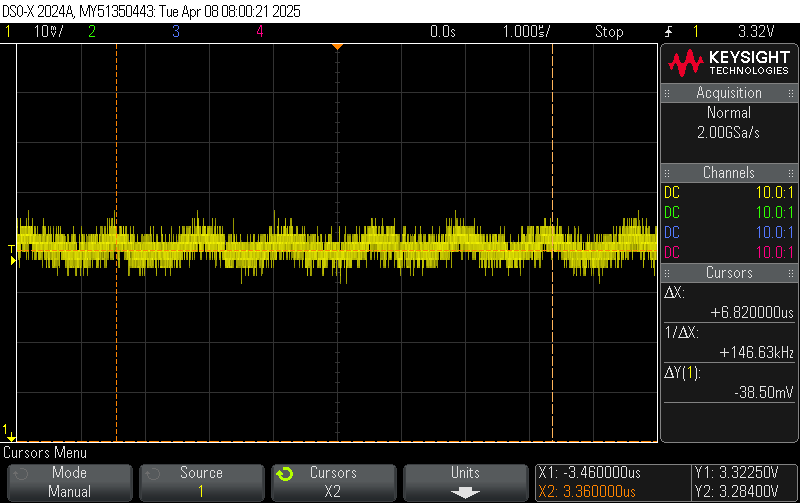
\includegraphics[height=6cm]{measurements/dcdc_ripple.png}
        \caption{Output ripple of the DC/DC converter}
        \label{fig:dcdc_ripple}
    \end{center}
\end{figure}
\FloatBarrier

\subsection{High Voltage power supply}
Next, the output voltage ripple of the high voltage power supply was measured at \SI{20}{\volt} with a \SI{100}{\kilo\ohm} load connected. The transient response to this load was also measured. 
\FloatBarrier
\begin{figure}[!htpb]
    \begin{center}
        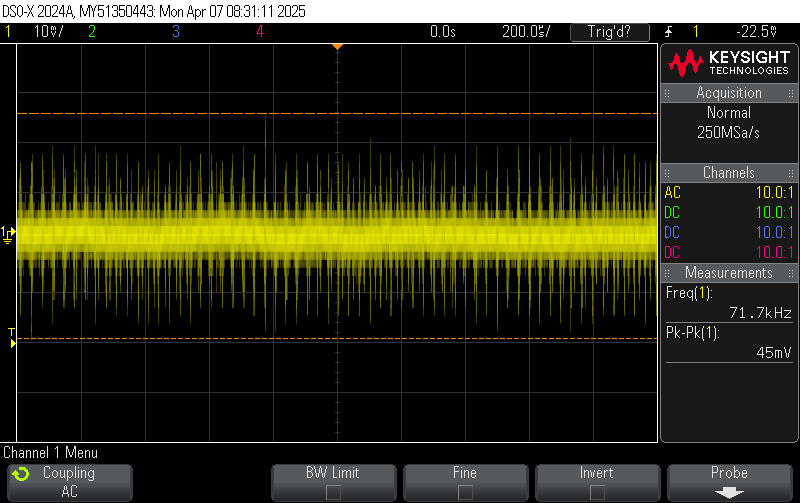
\includegraphics[height=6cm]{measurements/ripple.png}
        \caption{Output ripple of the high-voltage power supply}
        \label{fig:hv_ripple}
    \end{center}
\end{figure}
\FloatBarrier

\FloatBarrier
\begin{figure}[!htpb]
    \begin{center}
        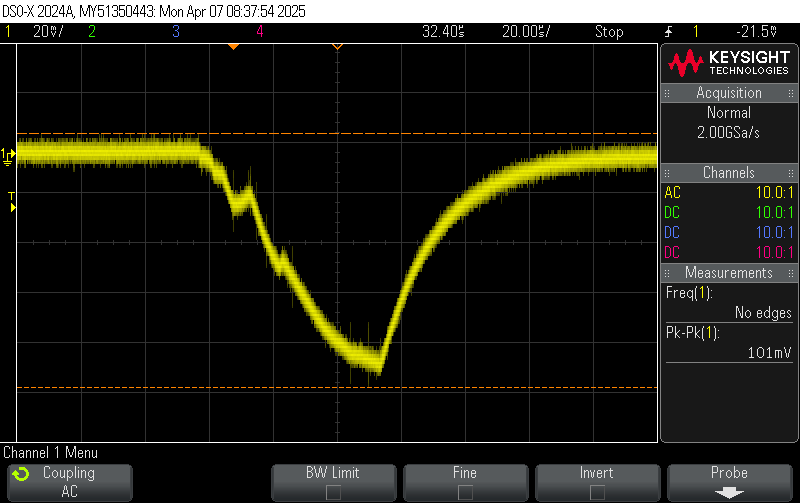
\includegraphics[height=6cm]{measurements/hv_transient.png}
        \caption{Trensient response of the high-voltage power supply}
        \label{fig:hv_transient}
    \end{center}
\end{figure}
\FloatBarrier

From Figure \ref{fig:hv_ripple}, it can be seen that a ripple of \SI{45}{\milli\volt} peak-to-peak was observed, which is low enough to avoid causing any issues with the biased sensors. These sensors will experience an even cleaner supply voltage due to the low-pass filtering. Figure \ref{fig:hv_transient} shows the transient response of the power supply. When the load is connected, the output voltage drops by \SI{100}{\milli\volt} and takes \SI{150}{\micro\second} to stabilize back to the setpoint. This will not cause any problems, as this voltage drop is small enough to avoid triggering any other sensors. The typical pulse from the connected sensor will also be much shorter, on the order of a few hundred nanoseconds, causing a much smaller voltage drop. Thus, the evaluated case represents a worst-case scenario.

\subsection{Pulse injection}
The function of the pulse injection circuitry was also verified by measurement, which can be seen in Figure \ref{fig:injection_meas}. The peak voltage of \SI{3.16}{\volt} corresponds to a current of approximately \SI{10}{\milli\ampere} through the front end. The width of the pulse was set to \SI{200}{\nano\second}.

\FloatBarrier
\begin{figure}[!htpb]
    \begin{center}
        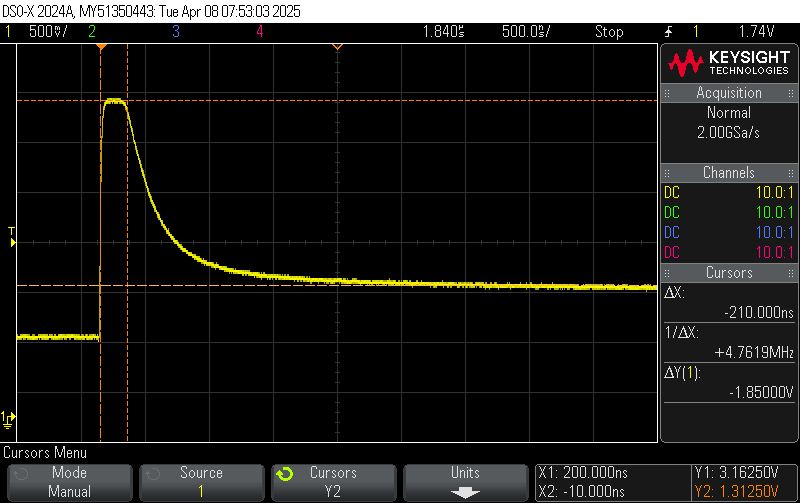
\includegraphics[height=6cm]{measurements/injection.png}
        \caption{Injected pulse}
        \label{fig:injection_meas}
    \end{center}
\end{figure}
\FloatBarrier

\section{Injection pulse test}
For the injection pulse test, the FastIC+ 1 was configured to enable the injection signal routing into channel 0. The injection pulse generator was than enabled to generate the injection signal (\SI{100}{\nano\second} pulses with \SI{100}{\micro\second} period). Streaming of the aurora data to the USB was than started and \SI{100}{\milli\second} capture of the bitsream was created. The python library was than used to parse the raw data into packets. The packets for a first packet detection is presented bellow.
\begin{small}
\begin{verbatim}
    --- Packet 1 ---
    Channel: 0
    Packet Type: PKT_TOTLN
    Timestamp absolute: 107474.438 us
    Pulse Width: 106.249 ns
  
    --- Packet 2 ---
    Channel: 8
    Packet Type: PKT_TOA_TOTNL
    Timestamp absolute: 107474.251 us
    Pulse Width: 1032.812 ns
  
    --- Packet 3 ---
    Channel: 0
    Packet Type: PKT_TOA
    Timestamp absolute: 107474.247 us
    Pulse Width: 124.218 ns

\end{verbatim}
\end{small}
\newpage
Along with a second detection that is subsequent to the fist one.
\begin{small}
\begin{verbatim}
    --- Packet 1 ---
    Channel: 0
    Packet Type: PKT_TOTLN
    Timestamp absolute: 107572.038 us
    Pulse Width: 107.031 ns
  
    --- Packet 2 ---
    Channel: 8
    Packet Type: PKT_TOA_TOTNL
    Timestamp absolute: 107571.850 us
    Pulse Width: 1035.546 ns
  
    --- Packet 3 ---
    Channel: 0
    Packet Type: PKT_TOA
    Timestamp absolute: 107571.846 us
    Pulse Width: 125.000 ns
  
\end{verbatim}
\end{small}

The two packets received on channel 0 correspond to the \emph{ToA} of the pulse, transferred in the \verb|PKT_TOA| packet, and the \emph{ToT} transferred in the \verb|PKT_TOTLN|. The third packet on channel 8 is the \emph{ToA} of the trigger pulse generated to start the FSM. These differ due to different thresholds and processing on the separate paths. Taking the relevant information from the first set, it can be seen that a packet with a \emph{ToT} of \SI{106.249}{\nano\second} was detected at time \SI{107474.247}{\micro\second}. The \emph{ToT} corresponds nicely to the generator pulse width. Taking the difference between the \emph{ToA} timestamps of the subsequent detections, the period of the pulses can be calculated as $T = \SI{107571.846}{\micro\second} - \SI{107474.247}{\micro\second} = \SI{97.599}{\micro\second}$, which corresponds to the set period of \SI{100}{\micro\second} of the injection generator. The inaccuracy of both the \emph{ToA} and \emph{ToT} originates from the injection generator rather than the FastIC+, which is very precise. The purpose of the injection is to easily check that the FastIC+ can receive pulses and process them correctly, rather than verifying the FastIC+'s accuracy. 


\section{SiPM SPTR measurement}
To verify the device's functionality in a real-world application and stress test the FastIC+ accuracy, a Single Photon Time Resolution (SPTR) measurement with a real SiPM was performed at CERN. In this test, a laser source sends short pulses of light to a \emph{SiPM} sensor connected to the readout. A trigger signal output from the laser is fed into the readout trigger input. On every laser shot, the readout is triggered by the laser and thus generates a \emph{ToA} packet on channel 8. After the beam of light travels to the \emph{SiPM}, it is converted into an electrical pulse and sensed by the FastIC+, which generates the \emph{ToA} and \emph{ToT} packets for the detection. The delay between the trigger \emph{ToA} and the detection \emph{ToA} corresponds to the time the \emph{SiPM} needs to detect the photon and generate the electrical pulse, thus the \emph{SPTR} of the \emph{SiPM}. The \emph{ToT} is used to detect only single-photon events. 
\\
\\
\large \textbf{TADY BUDE DALSI KOMENTAR K TOMU EXPERIMENTU AZ HO CERN UDELA :D}